\documentclass[10pt,a4paper,oneside]{article}
\usepackage[utf8]{inputenc}
\usepackage[ngerman]{babel}
\usepackage{amsmath}
\usepackage{amsfonts}
\usepackage{amssymb}
\usepackage{graphicx}
\author{Jeremias Eppler, Jochen Morent, Georgi Georgiev}
\title{Projektcontrolling Theorie}
\begin{document}
\maketitle
\section*{Projektcontrolling}
Beim Projektcontrolling vergleicht man in festgelegten Kontrollintervallen den Soll- und Ist-Zustand des Projektes.
Jeder Vergleich stellt also ein Kontrollpunkt dar. Sollte, bei einem Kontrollpunkt eine Abweichung zwischen Soll- und Ist-Zustand auftretten, dann sollte der Projekverantwortliche die Abweichungen deutlich kennzeichnen, z. B. im Termin, Balkenplan, Meilensteinplan usw. eintragen (Adaptieren). Die Abweichungen sollten mit dem gesamten Team besprochen und Korrekturmaßnahmen erarbeitet werden.
Wenn die Abweichungen zu groß sind, dann sollte eine Neuplanung des Projekts durchgeführt werden.
Die Abweichungen sollten in das Projekthandbuch aufgenommen werden. Darauf folgt das erstellen von Projektcontrolling berichten.
Anschließend werden die Maßnahmen koordiniert umgesetzt und die Projektdurchführung fortgesetzt. 

\begin{figure}[!ht]
\includegraphics[width=\textwidth, height=\textheight, keepaspectratio, angle=0]{image/projekcontrolling-zyklus}
\caption{ Projektcontrolling-Zyklus}
\end{figure}

Unter Projektkontrolling versteht man also die Überwachung und Neuanpassung des Projekts innerhalb von definierten Kontrollintervallen. Es handelt sich also um einen kontinuierlichen Prozess, der als Projektkontrollingprozess bezeichnet wird.
Das Projektcontrolling ist mit dem Projektcontrollingprozess flexibel genug um auf die dynamik, des sich ständig verändernden, Projektes zu reagieren.
Obwohl sich auch die Umwelt des Projektes Massiv ändern kann, sind bei der
Organisation des Projektcontrollingprozesses die Rollenträger des Projektes beteiligt und nicht die projekexternen Stellen\footnote{(Vgl. "Happy Projects!" 3. Auflage S. 180, Manz Verlags- und Universitätsbuchhandlung GmbH, Wien 2006)}, wie z. B. die Bereichs-Controller. An dem Projektcontrollingprozess ist der Projektmanager, das Projektauftraggeberteam und das Projektteam beteiligt.

\paragraph{ Wie lange sollte der Abstand zwischen den Kontrollpunkten sein? } ~\\

Das Projektcontrolling wird in festgelegten Intervallen vom Projektmanager immer wieder Durchgeführt. Eine projektangepasste Intervalllänge ist deshalb wichtig. Ist die Intervalllänge zu lang werden Misstände erst zu spät erkannt.
Ist das festgelegte Intervall zu kurz, ist das gesamte Projekt mehr mit der Projekneuplanung als mit der Projektdurchführung beschäftigt. Es ist also darauf zu achten die richtige Intervalllänge zu wählen. 
Beim Anlagebau der zwei Jahre dauert, könnte z. B. alle 6-8 Wochen ein Projektcontrolling durchgeführt werden. Bei projekten mit einer geringeren Laufzeit, sollte in kürzeren Abständen ein Projekcontrolling
stattfinden.
Desweiteren bietet es sich an ein Projektcontrolling beim erreichen von Meilensteinen zu veranschlagen.

\paragraph{ Woher kommen die Soll- und Istwerte? } ~\\

Ein Projekt beginnt mit dem Planen der Projektdurchführung, während des Planungsprozesses werden, z. B. die Terminpläne und Meilensteine festgelegt. Die, aus dem Planungsprozess, resultierenden Werte werden als Sollwerte des ersten Projektcontrollings verwendet und mit dem tatsächlichen Projekt-Ist-Zustand vergliechen. Der Ist-Zustand fließt in die Projekt(neu)planung mit ein. Das heißt eine Verschmelzung beider Werte findet statt. Beim nächsten Projekcontrolling werden also nicht die Anfangswerte, sondern die verschmolzenen Werte verwendet.

\paragraph{ Wozu braucht man Projekcontrolling überhaupt? } ~\\

Oft wird professionelles Projektcontrolling nur bei finanziel riskanten Projekten eingesetzt\footnote{(Vgl. "Happy Projects!" 3. Auflage S. 179, Manz Verlags- und Universitätsbuchhandlung GmbH, Wien 2006)}. Allerdings ist es auch bei kleineren bzw. weniger riskanten Projekten notwendig ein proffessioneles Projektcontrolling durchzuführen. Weil der Projektcontrollingprozess ein Projekt kontrolliert und steuert und dafür sorgt, dass die Projektziele effizient erreicht werden und jeder Projektbeteiligte 
informationen über den Projektstand erhält.
\end{document}